\documentclass[14pt]{extarticle}
\usepackage[utf8]{inputenc}
\usepackage[T1]{fontenc}
\usepackage{setspace}
\usepackage[margin=1in]{geometry}
\usepackage{hyperref}
\usepackage{graphicx}
\usepackage{booktabs}
\usepackage{helvet}
\usepackage{float}

\doublespacing

\title{Event-Driven Process Mining for Failure Cascade Detection in Vehicle Telemetry Systems}
\author{Garrett Gruss}
\date{February 21, 2026}

\begin{document}

\maketitle

\section*{Abstract}

This project applies process mining to motorsport vehicle telemetry to automate discovery of failure propagation patterns. Sensor signals are classified into discrete events using the SHIP safety state model, organized into time-windowed cases, and analyzed via Directly-Follows Graphs (DFGs) using the PM4Py library. Applied to the UCONN FSAE 2016 Endurance dataset (190,587 samples, 76 channels, 31 minutes), the pipeline detects 801 SHIP events across six subsystems, generates 404 cases, and produces DFGs revealing cross-subsystem event sequences without manual annotation.

\section{Introduction and Background}

This project provides a data-driven analysis using the UCONN FSAE 2016 dataset. A config-driven pipeline --- \texttt{EventClassifier} $\rightarrow$ SHIP Dispatcher $\rightarrow$ \texttt{CaseGenerator} $\rightarrow$ PM4Py --- classifies sensor transitions using the SHIP safety model~\cite{bishop1995}, labeling crossings into anomalous regimes as \textit{error activation} and returns to normal as \textit{error recovery}. Repeating failure-preceding sequences surface as high-frequency DFG edges~\cite{vanderaalst2004} without requiring a domain expert to search for them.

\section{Related Work}

Guralnik and Srivastava~\cite{guralnik1999} present batch and incremental algorithms for detecting events as change points in a signal's generative model. The \texttt{EventClassifier} implements analogous primitives --- threshold crossing, boolean state change, and local extrema --- using static, domain-calibrated thresholds rather than likelihood-based selection.

Bishop and Bloomfield~\cite{bishop1995} formalize the SHIP failure behavior model, defining five system states and six transitions. This project uses SHIP as a labeling framework: boolean threshold crossings produce False$\rightarrow$True (error activation) or True$\rightarrow$False (error recovery) tags, enabling the DFG to distinguish failure initiation from recovery paths.

Van der Aalst et al.~\cite{vanderaalst2004} introduce the Directly-Follows Graph as a process discovery primitive requiring no structural assumptions, making it appropriate for telemetry where failure pathways are unknown. PM4Py~\cite{berti2019} implements frequency and performance DFG variants; the latter annotates edges with mean inter-event timing. Van der Aalst et al.~\cite{vanderaalst2005} extend event log analysis to social networks; mapping subsystems to \texttt{org:resource} enables this as a stretch goal.

\section{Preliminary Data}

The dataset was pre-parsed from the AiM CSV export, yielding the properties in Table~\ref{tab:dataset}. Per-channel statistics (min, mean, max, percentiles) were computed to calibrate SHIP thresholds; Table~\ref{tab:thresholds} documents the key decisions. Several design-spec thresholds were replaced after inspection showed they never fired against the observed distributions. Two channels were found unusable: \texttt{roll angle\_unit} is populated with zeros throughout the session, and \texttt{f88.v batt\_v} does not exist in the parsed CSV (\texttt{battery\_v} is used instead).

\begin{table}[H]
\centering
\caption{Dataset Properties}
\label{tab:dataset}
\begin{tabular}{ll}
\toprule
Property & Value \\
\midrule
Rows & 190,587 \\
Channels & 76 \\
Sample rate & $\sim$100\,Hz \\
Duration & 1,905.5\,s ($\approx$31.8\,min) \\
\bottomrule
\end{tabular}
\end{table}

\begin{table}[H]
\centering
\caption{Threshold Calibration from Channel Distributions}
\label{tab:thresholds}
\begin{tabular}{lrrrr}
\toprule
Channel & Min & Mean & Max & Threshold \\
\midrule
Coolant temp (°F)   & 0      & 148  & 169  & $>160$\,°F        \\
Oil pressure (psi)  & $-0.8$ & 30.7 & 90.6 & $<5$ / $>80$\,psi \\
Battery voltage (V) & 12.9   & 13.9 & 15.0 & $<13.2$\,V        \\
GPS satellites      & 7      & ---  & 11   & $<8$\,sat          \\
Bumpstop (unit)     & 0      & 0.35 & 5.0  & $>0.0$             \\
\bottomrule
\end{tabular}
\end{table}

Several design-spec thresholds were replaced after inspection showed they never fired against the observed distributions. The coolant temperature design spec of 220\,°F was never reached (session max 169\,°F); 160\,°F was chosen to capture the observed high-temperature tail. For oil pressure, a 15\,psi lower bound flooded the log during low-RPM operation; 5\,psi separates genuine pressure drops from normal idle behavior, and 80\,psi catches anomalous spikes near the session maximum. Battery voltage remained stable throughout (std 0.43\,V), making the 11.5\,V design spec unreachable; 13.2\,V catches brief sags below the 1st percentile. GPS satellite count ranged from 7 to 11, so the 4-satellite spec never fired; $<8$ captures the observed session minimum. Bumpstop channels are binary in practice---0 (no contact) or 5 (full contact)---so any non-zero value indicates engagement.

The dispatcher ran 16 config entries over the full dataset; Table~\ref{tab:events} shows the results. Lubrication dominates at 68\% of events due to oil pressure cycling during low-RPM operation. The 404 error activation events were used as case triggers, producing 10,727 event-case assignments across 404 cases (avg 26.6 events/case) with a 10\,s pre-trigger and 30\,s post-trigger window.

\begin{table}[H]
\centering
\caption{SHIP Events Detected by Subsystem}
\label{tab:events}
\begin{tabular}{lrrr}
\toprule
Subsystem & Error Activation & Error Recovery & Total \\
\midrule
Suspension   & 72  & 72  & 144 \\
Brakes       & 3   & 0   & 3   \\
Engine       & 45  & 44  & 89  \\
Lubrication  & 274 & 274 & 548 \\
Electrical   & 7   & 7   & 14  \\
Drivetrain   & 3   & 0   & 3   \\
\midrule
\textbf{Total} & \textbf{404} & \textbf{397} & \textbf{801} \\
\bottomrule
\end{tabular}
\end{table}

\begin{figure}[H]
\centering
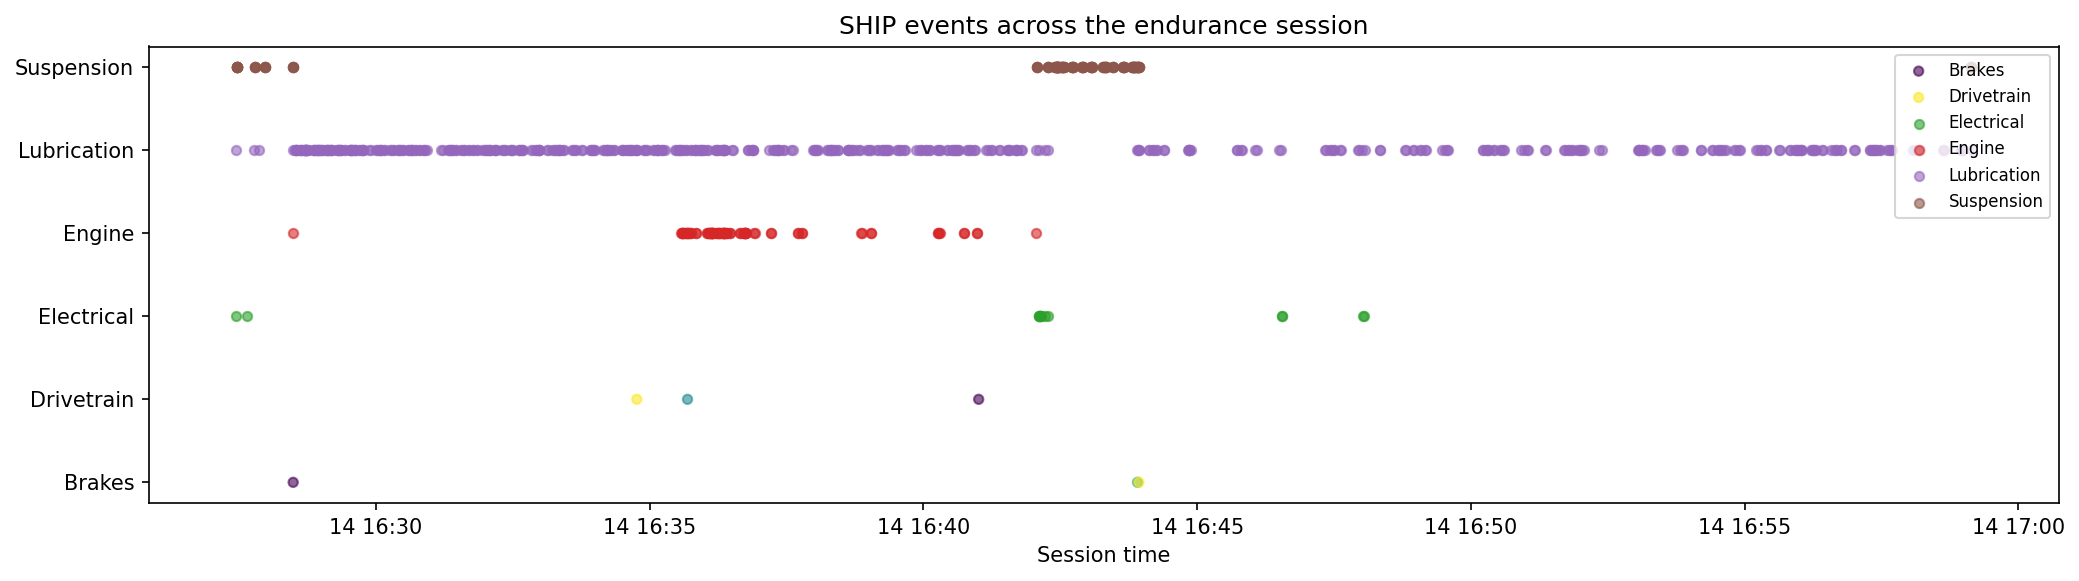
\includegraphics[width=\linewidth]{../../examples/example_5/data/processed/ship_events_timeline.png}
\caption{SHIP events across the 31-minute endurance session, grouped by subsystem.}
\label{fig:timeline}
\end{figure}

\begin{figure}[H]
\centering
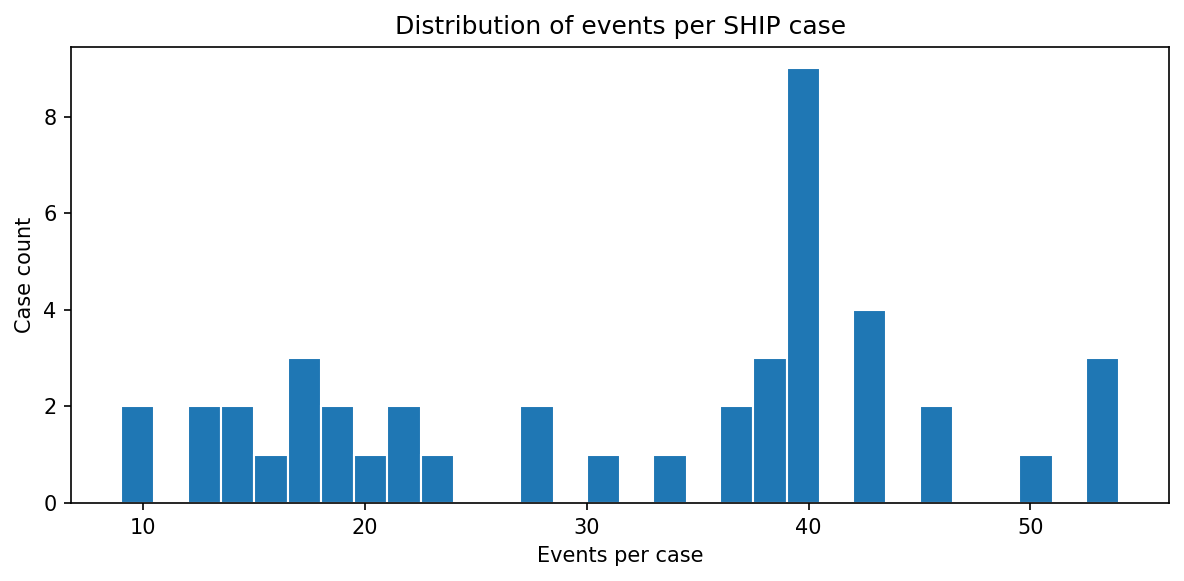
\includegraphics[width=0.8\linewidth]{../../examples/example_5/data/processed/ship_events_per_case.png}
\caption{Distribution of events per time-windowed case (404 cases, avg 26.6 events/case).}
\label{fig:epcase}
\end{figure}

Variant analysis identifies 201 unique event sequences. The most frequent variant (23 cases) is an isolated lubrication activation-recovery pair. The next most common variants pair Lubrication events with Suspension bumpstop hits, consistent with a load-transfer mechanism where hard cornering simultaneously engages the bumpstops and drops oil pressure. Lubrication dominance compresses DFG edge weights and may obscure rarer cross-subsystem interactions; subsystem filtering is planned for the next analysis phase.

\section{Work Remaining}

The core pipeline is complete and producing results. The following work remains before the final report.

\textbf{Subsystem filtering and threshold sensitivity.} Lubrication events dominate 68\% of the event log, compressing DFG edge weights and obscuring rarer cross-subsystem interactions. A subsystem-filtered DFG and sensitivity analysis across oil pressure thresholds will determine whether the dominance reflects genuine system behavior or an over-sensitive threshold.

\textbf{Window-size sensitivity analysis.} The 10\,s pre-trigger and 30\,s post-trigger window parameters directly determine which events appear in each case. Varying these parameters and comparing the resulting DFGs will establish how sensitive the variant structure is to window size and identify the range that best captures failure propagation without introducing unrelated events.

\textbf{SNA sociogram (stretch goal).} The \texttt{org:resource} field is already populated with subsystem labels in the PM4Py event log. Applying van der Aalst et al.'s handover-of-work and joint-case metrics~\cite{vanderaalst2005} would produce a sociogram showing which subsystems most frequently co-occur in failure cascade sequences.

\textbf{Final documentation and presentation.} Results from the above analyses will be compiled into the project report and presentation slides due in the final week.

\bibliographystyle{plain}
\bibliography{references}

\end{document}
